% !TEX root = ../paper.tex

\section{Case Study}

Our case study used the Qt project review history from the Gerrit code review tool provided by Hamasaki et. al. \cite{Hamasaki2013}. Qt project is a large open source project composed of numerous small subsystems. We selected the most active subproject, which is called \texttt{qtbase}.
From this subproject, we used the review history from May 2011 to June 2012, which contains 6,605 changes and 72,484 comments.


\subsection{Data Preparation}
We used the commit messages and comments in the dataset.
Before classifying the usefulness of comments, we first processed the commit message and comments as follows: 

\subsubsection{Removal of automatically generated messages} To consider only reviewers discussion, we ignored all messages that automatically generated.
%In Gerrit, the comment history is composed of human-written comments from reviewers and automatically generated messages.
These automatic messages are generated by Gerrit, continuous integration system, and the sanity bot\footnote{It is a bot that automatically checks new proposed changes for trivial sanity issues, such as line endings, copyright notices, and commit messages} to record activities. For example, \textit{`Upload patch set 1.'}, \textit{`Change has been successfully cherry-picked to the staging branch as ...'}, and \textit{`Sanity review passed'}. In practice, they are not considered in code review  and are not substantially relevant to the proposed changes and do not directly impact software quality\cite{Mcintosh}. 

To do so, we first ignore all comments written by bots i.e. \emph{Qt Continuous Integration System} and \emph{Qt Sanity Bot}. Second, we removed message including reviewers comments by finding common patterns frequently occurred using regular expression. This would leave us only human-written comments that will be used in further preprocessing.

%, . and hence are useless by our definition.
%%They are easily determined as useless by our method and would artificially improve our classification performance.
%These messages are identified by looking for the most common lines of text using regular expression.
%%Regular expression patterns are then constructed to match and remove these messages.
%Occurrences of these patterns are then removed from our dataset prior to further preprocessing.
%
%Automatic messages are also often inserted as part of review comments.
%They too are removed from our dataset, leaving us with only human-written part.
%We also completely ignored comments whose author is \emph{Qt Continuous Integration System} and \emph{Qt Sanity Bot}.

\subsubsection{Data preprocessing}
As is customary for VSM processing, we extracted semantic words from commit messages and comment messages before converting to vector.
For each message, we removed all punctuation signs (except apostrophe) and other non alphanumeric characters. We also removed common words (e.g. a, an, the) using Google stop word list\footnote{Available at \url{http://meta.wikimedia.org/wiki/Stop_word_list/google_stop_word_list#English}}. We then used Porter stemming algorithm to remove the commoner morphological and inflexional endings from words in English.

Table \ref{tb:datastatistic} summarizes data set we used for this study after preparation. 

\begin{table}[!h]
\caption{A summary data sets and some statistics.}
\centering
\small
\begin{tabular}{ccc}
\hline
& Total Number & Percentage \\ \hline \hline
Commit Messages & 6,605 &  -  \\ \hline
All Comments & 72,484& - \\ \hline
Reviewers Comments & 10,583 & 15\% \\ \hline
Automated Comments & 61,814 & 85\% \\ \hline 

\end{tabular}
\label{tb:datastatistic}
\end{table}
\subsection{Manual Comment Usefulness Assessment}
In this case study, three participants (the first two authors and one student) independently classify comments by giving a question that “Does this comment technically contribute to its change or not?”. Then, the participants gave a vote for \texttt{YES} if the comment is likely to useful and  \texttt{NO}  if the comment is likely to useless. From the voting scores, we regarded that the comments with three  \texttt{YES}  votes are \emph{useful} comments and the comments with no  \texttt{YES}  votes (i.e. three  \texttt{NO}  votes) are \emph{useless} comments. For the comments with one and two YES’ votes, we defined them as unclear comments.

\subsection{Research Questions}
We addressed two research questions: \textbf{RQ1:} Is semantic similarity a good indicator of MCR comment usefulness? and \textbf{RQ2:} Is semantic similarity classification cost-efficient, assurable, and scalable?.
\pick{Do we need motivation for these RQs?}
%\pick{I realize that your figure is better for the presentation :)}
%\begin{figure}[h]
%\centering
%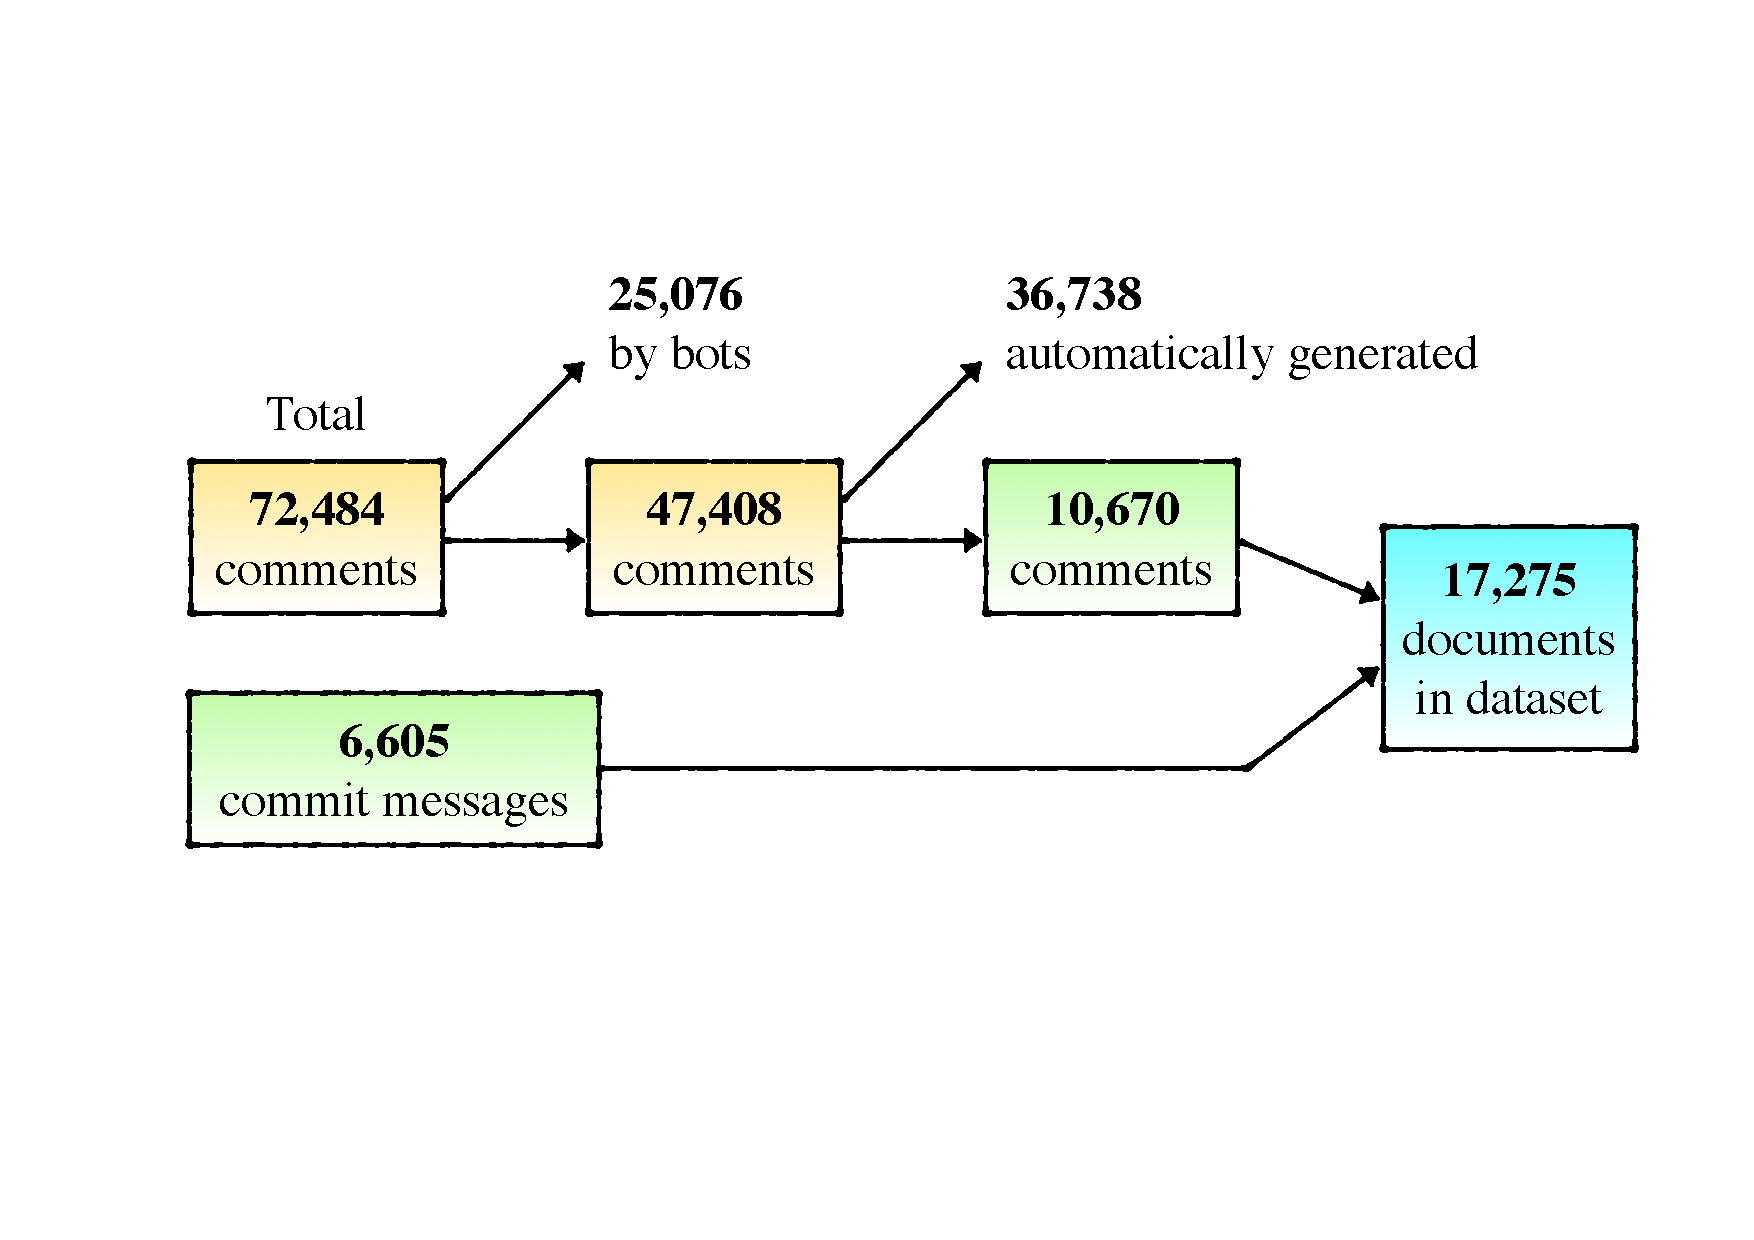
\includegraphics[width=3.2in]{filter}
%\caption{The filtering process.}
%\label{fig:filter}
%\end{figure}
%\subsection{Data Preparation}
%\subsubsection{Data extraction}
%
%6,605 changes and 72,484 comments have been extracted from the raw dataset.
%35\% of the comments are by the system or one of the bots, and are thus discarded.
%
%\subsubsection{Common pattern removal}
%
%By looking for most frequent lines, common patterns were found, such as \emph{`Uploaded patch set 2.'} and \emph{`Change has been successfully cherry-picked to the staging branch as \dots'}.
%
%Removing occurrences of these patterns leaves 77\% of the remaining comments empty.
%This probably means these comments solely contain automatically-generated text, and are thus discarded.
%This leaves us with 10,670 comments and 6,605 commit messages; a total of 17,275 documents.
%
%\subsubsection{Tokenizing}
%
%After the tokenization step, 393,238 tokens are generated in total. They are composed of 20,025 different words.
%This means that each document will be converted into a vector of 20,025 dimensions, each dimension representing a single word.


\begin{ResearchQuestions}
\item[RQ1:] Is semantic similarity a good indicator of MCR comment usefulness?
\end{ResearchQuestions}

\begin{figure}[!t]
\centering
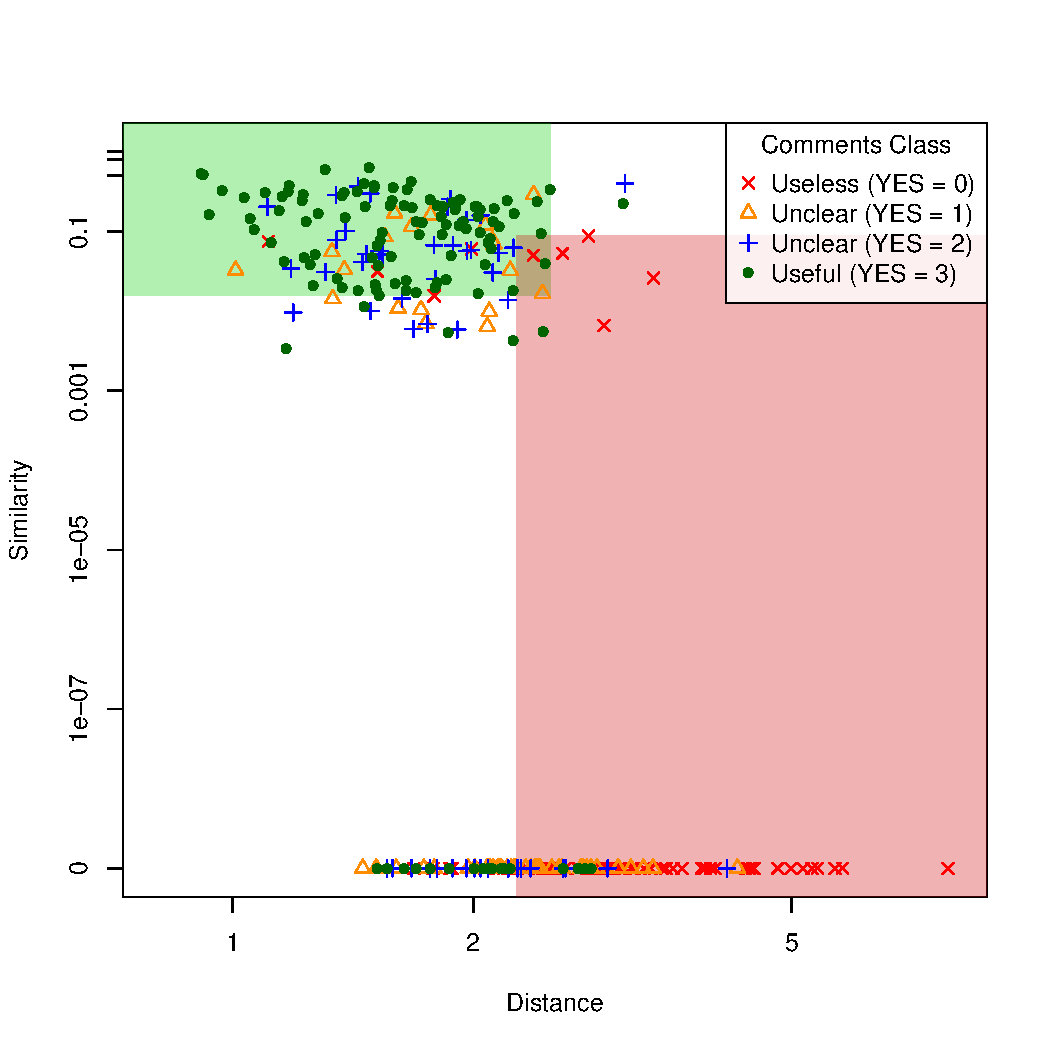
\includegraphics[scale=0.45, trim=0 0 30 50, clip=true]{scatter_log}
\caption{The similarity and distance plot of the training data.
The symbol represents the score, which ranges from 0 to 3.}
\label{fig:scatter}
\end{figure}

To answer this question, we randomly sampled 318 comments from our data set and manually identified usefulness.
Then, we used these comments for both the training and test data set for our approach to determine its effectiveness.
We also determined the effectiveness of our approach using bootstrapping cross validation.

% \dan{What what the effort in person-hours for this?}
% Thai sez:  Average time per comment is 28 seconds.
%            Since we do a lot of other things while training, it gives us a STDEV of 45 seconds.
%            The median, by the way, is just 10 seconds.

% Since our models do not include unclear type of comments, we defined them as negative condition i.e useless comments in case of useful classification (when using $\Theta(c,S_T,D_T)$ model) and useful comments in case of useless classification (when using $\Omega(c,S'_T,D'_T)$ model).
%\dan{I thought we changed this! It would be bad if we didn't. Let me know what the actual situation is here.}
%
% Thai sez:  We did not. Maybe this is just a matter of wording. I believe what the text says is:
%                - For useful classification, we only look for 3 scored comments.
%                - For useless classification, we only look for 0 scored comments.

To determine similarity and dissimilarity thresholds for useful and useless model, we iterated $s_t$ and $d_t$ values from every unique similarity and dissimilarity values in our data set.
%Table \ref{tb:thresholds} shows 5 sets of thresholds that best classify useful and useless comments based on F$_1$ score.
We selected the thresholds that best classify useful and useless comments based on F-measure score and applied models, i.e. useful: $\Theta(c,S_T=0.015529,D_T=2.494944)$ and useless: $\Omega(c,S_T=0.087522,D_T=2.265679)$ on the samples. 



\textbf{Model Effectiveness Results:} From 318 samples, the number of labeled comments were 85, 60, 51, and 122 for 0, 1, 2, and 3 \texttt{YES} votes, respectively. The precision and Recall of the models are 0.701 and 0.787 for useful model and 0.648 and 0.824 for useless model. We summarizes the number of classification from result described in Table \ref{tb:classify_number}.  We also show the results and relationship between comments class that manually classified and the similarity thresholds in Fig  \ref{fig:scatter}. The green area represents the \emph{useful} classification model and the red area represents the \emph{useless} model. Thus, the comments drawn in the green area are those satisfied condition of useful model and the comments drawn in the red area are those satisfied condition of useless. While, the comments drawn in the white area are those not satisfied any condition (i.e. undetermined). 
%This figure also shows an example comment that fall in the different area\pick{Didn't put yet}.


%%Interpret: comments & model%%%%
As shown in the figure, most comments drawn in green area are useful and very few useless comments drawn in this area. Similarly, most comments in the red area are useless. The unclear comments are drawn in both area. Between these areas, there is an overlap section. This is because the similarity and dissimilarity values between useful and useless are vague. Both models tend to maximize coverage of classification. Thus, it is possible that there is overlap between these two models. However, from the results in Table \ref{tb:classify_number}, only three comments were classified overlap section. This shows that error of our models is low. Furthermore, there are 12 useless comments  (14\%) and  21 useful comments (17\%) still are undetermined (drawn in white area). We investigate characteristics of these comments. The findings are described in our discussion section.
%From the example comment, it shows that these comments discussed on \TODO{insert topic}, but did not contain any word in common.

\begin{table}[!t]
\centering
\small
\caption{Number of comments classified by our approach against ground truth data}
\begin{tabular}{ccccc}
\hline
& \multicolumn{4}{c}{Class from Manual Assessment} \\ \cline{2-5}
Our&  Useless  & Unclear  & Unclear & Useful \\
Classifications&  (\texttt{YES}=0) & (\texttt{YES}=1) & (\texttt{YES}=2) & (\texttt{YES}=3) \\
\hline \hline
Useful & 3 & 12 & 24 & 94 \\
Useless & 69 & 23 & 7 & 6 \\
Overlap & 1 & 1 & 0 & 1 \\
Undetermined & 12 & 24 & 20 & 21 \\
\hline
\end{tabular}
\label{tb:classify_number}
\end{table}

%%Interpret: comments & similarity values%%%%
The graph also shows that the useful comments have less distance (not higher than 3 approximately) while most of useless comments have zero similarity. However, the unclear comments are still spread out over the graph which we cannot determine relationship between their similarity.
Furthermore, it is interesting that comments can be clearly separated into two major groups: comments with high similarity values and comment with zero similarity. This indicates that the comments  in each group have relationship other than similarity. This led us to investigate insight into these comments to find other properties in our future work. 




Interestingly, in Table \ref{tb:classify_number}, there are 88\% of useful comments classified by our model have \texttt{YES} = 2 and 3 voting scores. The classification of useless comments also have similar proportion i.e. having high number of comment with \texttt{YES} = 0 and 1 voting scores. As the manual classification can be subjective, these comments were not received three voting scores.  It is possible that the unclear comments with \texttt{YES} = 2 can be useful comments and comments with can be useless comments. 


%\begin{table*}[!t]
%\caption{An accuracy of similarity and dissimilarity thresholds for useful and useless comment classifications}
%\small
%\centering
%\def\arraystretch{1.2}
%\begin{tabular}{ccccccc}
%\hline
%Prediction Models  & Rank & $s_t$ & $d_t$ & F-measure & Precision & Recall \\ \hline \hline
%\multirow{5}{*}{\textbf{useful}: $\Theta(c,S_T=s_t,D_T=d_t)$}
%& 1 & 0.015529 & 2.494944 & 0.741 & 0.701 & 0.787 \\ \cline{2-7}
%& 2 & 0.015529 & 3.077129 & 0.740 & 0.693 & 0.795 \\ \cline{2-7}
%& 3 & 0.016713 & 2.494944 & 0.739 & 0.704 & 0.779 \\ \cline{2-7}
%& 4 & 0.015411 & 2.494944 & 0.738 & 0.696 & 0.787 \\ \cline{2-7}
%& 5 & 0.015411 & 3.077129 & 0.738 & 0.688 & 0.795
%% \\ \cline{2-7}
%% & \multicolumn{3}{r}{Average} &  1.00 & 1.00 & 1.00 \\ \cline{2-7}
%%& \multicolumn{3}{r}{Min-Max} &   1.00 - 1.00 & 1.00 - 1.00  & 1.00 - 1.00
%\\ \hline \hline
%\multirow{5}{*}{\textbf{useless}: $\Omega(c,S'_T=s_t,D'_T=d_t)$}
%& 1 & 0.087522 & 2.265679 & 0.725 & 0.648 & 0.824 \\ \cline{2-7}
%& 2 & 0.087522 & 2.250422 & 0.722 & 0.642 & 0.824 \\ \cline{2-7}
%& 3 & 0.087522 & 2.324771 & 0.720 & 0.663 & 0.788 \\ \cline{2-7}
%& 4 & 0.052856 & 2.265679 & 0.719 & 0.645 & 0.812 \\ \cline{2-7}
%& 5 & 0.087522 & 2.249675 & 0.718 & 0.636 & 0.824
%% \\ \cline{2-7}
%%& \multicolumn{3}{r}{Average} &  1.00 & 1.00 & 1.00 \\ \cline{2-7}
%%& \multicolumn{3}{r}{Min-Max} &   1.00 - 1.00 & 1.00 - 1.00  & 1.00 - 1.00
%\\ \hline
%\end{tabular}
%\label{tb:thresholds}
%\end{table*}

\begin{table*}[!t]
\caption{Results from bootstrapping cross validation of our classification models against random models}
\small
\centering
\def\arraystretch{1.2}
\begin{tabular}{cccc|cc|cc}
\hline
\multicolumn{2}{c}{Classifcation}   & \multicolumn{2}{c|}{Precision} & \multicolumn{2}{c|}{Recall} & \multicolumn{2}{c}{F-measure} \\ \cline{3-8}
\multicolumn{2}{c}{Models} & Avg. & STD. & Avg. & STD. & Avg. & STD. \\ \hline \hline
\multirow{2}{*}{Useful} & $\Theta(c,S_T,D_T)$    &  0.654 & 0.116 &  0.759 & 0.123 & 0.693 & 0.089\\ \cline{2-8}
& Random     &  0.421 & 0.114 &  0.376 & 0.116 & 0.496 & 0.144\\ \hline
\multirow{2}{*}{Useless}  & $\Omega(c,S'_T,D'_T)$  &  0.636 & 0.144 &  0.755 & 0.148 & 0.681 & 0.118\\ \cline{2-8}
& Random    &  0.336 & 0.131 &  0.269 & 0.115 & 0.478 & 0.182\\
\hline
\end{tabular}
\label{tb:xvalidate}
\end{table*}


\textbf{Validation:} We validated our approach using bootstrapping cross validation. We randomly selected 90\% of 318 comments for training set and determine thresholds. We then applied the constructed model on the remaining 10\% comments as the validation set.
The performance on the validation sets was measured using precision, recall and F-measure.
This validation was repeated for 300 times to estimate the performance of our models.
For a baseline of our models, we determined the performance of the random models using same methods.

Table \ref{tb:xvalidate} describes the performance of useful and useless classification models including an average and standard deviation of precision, recall, and F-measure. The results show that both of our models can achieve  60\% of precision and  75\% of recall approximately. Moreover, our models also achieved higher results than the random models twice for both precision and recall.


%\begin{table*}[!t]
%\caption{An accuracy of similarity and dissimilarity thresholds for useful and useless comment classifications}
%\small
%\centering
%\def\arraystretch{1.2}
%\begin{tabular}{ccccccc}
%\hline
%Prediction Models & $s_t$ & $d_t$ & F-measure & Precision & Recall \\ \hline \hline
%$\Theta(c,S_T=s_t,D_T=d_t)$   & 0.015529 & 2.494944 & 0.741 & 0.701 & 0.787 \\ \hline
%$\Omega(c,S'_T=s_t,D'_T=d_t)$ & 0.087522 & 2.265679 & 0.725 & 0.648 & 0.824 \\ \hline
%\end{tabular}
%\label{tb:thresholds}
%\end{table*}



According to the results, we can answer RQ1 that \emph{there is a relation between semantic similarity usefulness of comments. Based on our approach, the semantic similarity can be used as an indicator to classify usefulness of comments. 
}

%After we performed cross validation, we obtained the following result:
%for positive and negative classifications,
%we obtained an average F$_1$ score of 0.693 and 0.681,
%with standard deviation of 0.090 and 0.118, respectively.
%This indicates that we can use our approach to classify with confident of 69.8\%.

%After the similarity and distance metrics have been calculated,
%these metrics appear to be able to separate the useful comments from the non-useful ones,
%as can be seen in Fig.\ref{fig:scatter}.
%Note that many comments have a cosine similarity metric of 0.
%This is because the comment text and the corresponding commit message has no word in comment.






\begin{ResearchQuestions}
\item[RQ2:] Is semantic similarity classification cost-efficient, assurable, and scalable?
\end{ResearchQuestions}

To answer this question, timestamps are recorded as three people assess each comment.
Since three people work on their leisure time, there is much variability in the time between each vote.
Therefore, we ignored the time interval between two votes if they are more than 10 minutes apart.

On average, it takes 28 seconds to assess each comment.
However, the median is 10 seconds, suggesting that most comments take only a little amount of time to assess; only few comments take long time.
This also suggests that the time to assess each comment is not normally distributed.
The standard deviation is 45 seconds.

To estimate the total time for us to assess these 318 comments,
we multiplied the average time by the number of comments and the number of people.
This results in 7.42 person hours.

To manually assess all 10,583 comments---even with only one person working at 10 comments per minute---this would take 17.6 person hours.
By running our model through all 10,583 comments, only 2,487 comments receive undetermined result.
That means that about 77\% of the effort is saved.

\pick{Note from Dan sensei,}

For cpost effectivness we can state the reduction  percentage in the number of comments that much be checked manually.

 Also point out how much effort manual classification takes and that it is error prone (probably mor so than the automated method!
 
You cannot, but some estimates are possble

first, human beings have a fairly well known rate of making errors in classification

second, look at the comments in the training set that the method classified differently, especially the unclear.

Review these to see if the method suggested a better classification than was originally made by the assessors

You can consider these errors. Now look at what wans the percent of errors in the training set

This is also an estimate of the human error rate

















